\PassOptionsToPackage{unicode=true}{hyperref} % options for packages loaded elsewhere
\PassOptionsToPackage{hyphens}{url}
%
\documentclass[]{article}
\usepackage{lmodern}
\usepackage{amssymb,amsmath}
\usepackage{ifxetex,ifluatex}
\usepackage{fixltx2e} % provides \textsubscript
\ifnum 0\ifxetex 1\fi\ifluatex 1\fi=0 % if pdftex
  \usepackage[T1]{fontenc}
  \usepackage[utf8]{inputenc}
  \usepackage{textcomp} % provides euro and other symbols
\else % if luatex or xelatex
  \usepackage{unicode-math}
  \defaultfontfeatures{Ligatures=TeX,Scale=MatchLowercase}
\fi
% use upquote if available, for straight quotes in verbatim environments
\IfFileExists{upquote.sty}{\usepackage{upquote}}{}
% use microtype if available
\IfFileExists{microtype.sty}{%
\usepackage[]{microtype}
\UseMicrotypeSet[protrusion]{basicmath} % disable protrusion for tt fonts
}{}
\IfFileExists{parskip.sty}{%
\usepackage{parskip}
}{% else
\setlength{\parindent}{0pt}
\setlength{\parskip}{6pt plus 2pt minus 1pt}
}
\usepackage{hyperref}
\hypersetup{
            pdfborder={0 0 0},
            breaklinks=true}
\urlstyle{same}  % don't use monospace font for urls
\usepackage{graphicx,grffile}
\makeatletter
\def\maxwidth{\ifdim\Gin@nat@width>\linewidth\linewidth\else\Gin@nat@width\fi}
\def\maxheight{\ifdim\Gin@nat@height>\textheight\textheight\else\Gin@nat@height\fi}
\makeatother
% Scale images if necessary, so that they will not overflow the page
% margins by default, and it is still possible to overwrite the defaults
% using explicit options in \includegraphics[width, height, ...]{}
\setkeys{Gin}{width=\maxwidth,height=\maxheight,keepaspectratio}
\setlength{\emergencystretch}{3em}  % prevent overfull lines
\providecommand{\tightlist}{%
  \setlength{\itemsep}{0pt}\setlength{\parskip}{0pt}}
\setcounter{secnumdepth}{0}
% Redefines (sub)paragraphs to behave more like sections
\ifx\paragraph\undefined\else
\let\oldparagraph\paragraph
\renewcommand{\paragraph}[1]{\oldparagraph{#1}\mbox{}}
\fi
\ifx\subparagraph\undefined\else
\let\oldsubparagraph\subparagraph
\renewcommand{\subparagraph}[1]{\oldsubparagraph{#1}\mbox{}}
\fi

% set default figure placement to htbp
\makeatletter
\def\fps@figure{htbp}
\makeatother


\date{}

\begin{document}

\textbf{4. Автоколебания}

4.1. Автоколебания в системах с одной степенью свободы. В предыдущих
разделах были рассмотрены свободные и вынужденные колебания в
диссипативных системах с одной степенью свободы, подчиняющихся
дифференциальным уравнениям второго порядка вида (2.5) и (2.45)
соответственно. Диссипация энергии, обусловленная наличием резистивных
элементов в этих системах, в первом случае приводила к затуханию
колебаний, а во втором -- компенсировалась энергией, поступающей от
внешнего источника синусоидального напряжения (или тока). Однако
колебания в системе с одной степенью свободы при определённых условиях
можно поддерживать, используя постоянный (не синусоидальный) источник
энергии, который периодически компенсирует потери колебательной энергии
по входящей в систему цепи обратной связи. Такие системы называются
\textbf{автоколебательными}, а протекающие в них процессы --
\textbf{автоколебаниями}. Форма и период автоколебаний определяются
свойствами самой системы, чем автоколебания существенно отличаются от
колебаний вынужденных.

Для определения условий возбуждения автоколебаний в диссипативной
системе с одной степенью свободы запишем уравнение (2.5) с учётом формул
(2.2), (2.3) в виде

\begin{equation}\[\frac{dW}{dt}=-P(t),\label{eq:auto.1}\end{equation}

где \(W={L{{I}^{2}}}/{2}\;+{{{q}^{2}}}/{2C}\;\)-- энергия, запасённая в
колебательном контуре, а \(P(t)=R{{I}^{2}}(t)\)-- мощность потерь.
Интегрируя уравнение \ref{eq:auto.1} по периоду колебаний \(T\),
приходим к равенству

\begin{equation}W={{W}_{0}}-\int\limits_{0}^{T}{P(t)dt,\label{eq:auto.2}\end{equation}

где \({{W}_{0}}\)-- энергия системы в некоторый момент времени, принятый
за начало отсчёта периода колебаний \(T\). В обычной -- диссипативной --
системе \(P(t)>0\), так что автоколебания невозможны. Если же мощность
потерь \(P(t)=R{{I}^{2}}(t)\) в системе {знакопеременна}, то подбором
режима работы системы можно обеспечить энергетический баланс:

\begin{equation}\int\limits_{0}^{T}{R{{I}^{2}}(t)dt}=0,\label{eq:auto.3}\end{equation}
и, следовательно, возбудить в системе автоколебания.

Выполнение условия \ref{eq:auto.3} возможно, например, в {нелинейной}
колебательной системе, в которой сопротивление \(R\) является функцией
тока: \(R=R(I)\), причём -- {знакопеременной}. Необходимым для
автоколебательного режима отрицательным «сопротивлением» \({dV}/{dI}\)
на «падающих» участках своих вольт-амперных характеристик \(I(V)\),
представленных на рис.~11(а, б), обладают, например, газоразрядная лампа
(а) и туннельный диод (б). Обычно характеристики вида (а) называют
\emph{S}-образными, а вида (б) -- \emph{N}-образными.

\begin{figure}
\centering

\includegraphics{Images/media/image16.jpeg}
\caption{}
\end{figure}

а) б)

Рис.11. Вольт-амперные характеристики с «падающими» участками:

а) \emph{S}-образным, б) \emph{N}-образным

Форма автоколебаний зависит от добротности колебательного контура. При
большой добротности характер протекающих процессов почти не изменяется
по сравнению с тем, как они протекали бы в системе без поступления
энергии от источника: период и форма автоколебаний будут близки к
периоду и форме собственных колебаний. Это связано с тем, что в этом
случае от постоянного источника поступает энергия, составляющая малую
долю полной энергии колебательной системы. При малой добротности контура
(в общем случае -- колебательной системы) для поддержания колебаний от
постоянного источника должна поступать энергия, сопоставимая с энергией
колебаний. В этом случае форма автоколебаний может значительно
отличаться от синусоидальной. Наконец, в периодической системе, в
которой за период автоколебаний теряется вся накопленная энергия,
автоколебания становятся \textbf{релаксационными} и могут по форме очень
сильно отличаться от колебаний синусоидальных.

4.1. Автоколебания в вырожденных колебательных системах.
Автоколебательная система, не содержащая одного из накопителей
колебательной энергии, называется \textbf{вырожденной}. Колебания в
такой системе описываются дифференциальным уравнением первого порядка и,
очевидно, могут быть только релаксационными. В рассматриваемом здесь
случае электрических колебаний речь идёт об отсутствии в системе одного
из реактивных элементов: индуктивности или ёмкости.

В качестве примера рассмотрим представленную на рис.~12(а, б)
вырожденную колебательную систему, содержащую источник постоянного
напряжения \emph{U}, ёмкость \emph{C}, сопротивление \emph{R} и
нелинейный элемент с \emph{S}-образной вольт-амперной характеристикой
\({{I}_{S}}(V)\). Как видно, в системе отсутствует второй накопитель
колебательной энергии -- индуктивность.

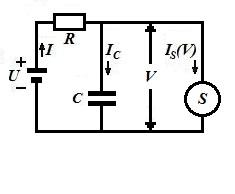
\includegraphics{Images/media/image18.jpeg}
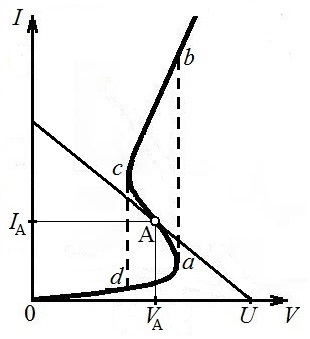
\includegraphics{Images/media/image19.jpeg}

\begin{quote}
а) Схема автоколебательной \emph{RC}-системы б) Вольт-амперная
характеристика и нагрузочная прямая
\end{quote}

Рис. 12(а, б). Вырожденная автоколебательная система

Уравнения, описывающие поведение этой системы релаксационного типа,
имеют вид:

\begin{equation} RI+V=U,\]    \[I={{I}_{C}}+{{I}_{S}},\]  \[{{I}_{C}}=C\frac{dV}{dt},\]   \[{{I}_{S}}={{I}_{S}}\left( V \right). \label{eq:auto.4}\end{equation}

Следовательно,

\begin{equation} RC\frac{dV}{dt}=U-V-R{{I}_{S}}\left( V \right).\label{eq:auto.5}\end{equation}

В стационарном состоянии, когда , должно выполняться равенство

\begin{equation} {{I}_{S}}(V)={(U-V)}/{R} \label{eq:auto.6}\end{equation}

Правая часть здесь представляет \textbf{нагрузочную} прямую, точки
пересечения которой с вольт-амперной характеристикой
\({{I}_{S}}\left( V \right)\) определяют стационарные состояния системы.
На рис.12б параметры \(U\) и \(R\) выбраны так, чтобы стационарное
состояние \(A({{V}_{A}},{{I}_{A}})\) лежало на падающей ветви
вольт-амперной характеристики, где, как говорилось выше, возможен
автоколебательный режим. Покажем, что состояние
\({{I}_{\text{}}}=I({{V}_{\text{}}})\) может быть {неустойчивым}. Для
этого дадим малое приращение \(v\) переменной \(V\) в точке
\({{V}_{A}}\) и представим в линейном приближении по \(v\)
вольт-амперную характеристику \(I(V)\) вблизи стационарного состояния
\(V_A\):

\begin{equation} I(V)=I({{V}_{\text{}}}+v)\approx I\left( {{V}_{\text{A}}} \right)+{I}'\left( {{V}_{\text{A}}} \right)v, \label{eq:auto.7}\end{equation}

где «штрих» означает производную по \emph{V}. Подстановка этого
выражения в \ref{eq:auto.5} приводит к уравнению

\begin{equation} RC\frac{dv}{dt}=-\left[ 1+R{I}'\left( {{V}_{\text{A}}} \right) \right]v, \label{eq:auto.8}\end{equation}

из которого следует, что при условии

\begin{equation} {I}'\left( {{V}_{\text{A}}} \right)<-{1}/{R}\label{eq:auto.9}\end{equation}

возмущение \(v\) со временем экспоненциально нарастает, и, значит,
стационарное состояние \({{I}_{\text{}}}=I({{V}_{\text{}}})\) является
неустойчивым. Система при этом будет совершать {релаксационные
автоколебания}, замкнутая фазовая траектория которых на рис. 12б состоит
из плавных участков \emph{da} и \emph{bc} вольт-амперной характеристики
между напряжениями \(V_1\) и \(V_2\), соединённых двумя вертикальными
участками \emph{ab} и \emph{cd}, показанными на рисунке штриховыми
линиями. Формально вертикальные участки соответствуют {скачкам тока},
которые возможны только при отсутствии индуктивностей в системе, исходно
заложенной в данной идеализированной модели. Учёт малой «паразитной»
индуктивности элементов схемы, приводящей к появлению э.д.с. индукции и,
соответственно, к конечной скорости скачков, добавляет ещё одно
дифференциальное уравнение первого порядка. Систему в целом теперь
описывает дифференциальное уравнение второго порядка, которое позволяет
получить периодическое решение, представляющее автоколебательный
процесс.

\end{document}
